%!TEX root = ../thesis.tex

\chapter[The Negacyclicity Problem]{Overcoming the negacyclicity problem with odd plaintext modulus}
\label{chap:negacyclicity}


In Section \ref{sec:pbs}, we presented the algorithm of the PBS. But we left a question unanswered: what is the actual composition of the accumulator polynomial $\acc$? This is a tricky question, because this definition depends on the countermeasure picked against the negacyclicity problem (that we briefly introduced in Section \ref{sec:overview_blind_rotation}). 


In this chapter, we formalize the negacyclicity problem. We then present the classical countermeasure (the strategy of the padding bit), and our technique of odd plaintext modulus, which is a foundational block for the following contributions presented in this thesis. We finish by going through several others works that propose different countermeasures.


\section{Basics on negacyclicity}

\paragraph{What is negacyclicity ?}

Let $v(X)$ be a polynomial of the ring $\glweRing$, such that $v(X) = \sum_{k=0}^{N-1} v_k X^k$. Recall how a multiplication by $X$  in this ring ``rotates'' the coefficients of the polynomial: \[X \cdot v(X) = - v_{N - 1} + v_0 \cdot X \dots + v_{N - 2} X^{N - 1}~.\]

In TFHE's blind rotation, the polynomial multiplication in the blind rotation is actually done by $X^{-\Tilde{\mu}}$, which lives in $\{0, \dots, 2N - 1\}$. This leads to two problems:

\begin{itemize}
	\item A coefficient $v_j$ can be brought in first place by two different rotations: the one induced by the polynomial multiplication by $X^{\modulo{-j}{2N}}$ and the one by $X^{[-j + N]_{2N}}$.
	\item Each time a coefficient goes last to first, it gets negated (because $X^N = -1$ in the ring). So actually, the multiplication by $X^{[-j]_{2N}}$ yields correctly $v_j$, but the one by $X^{[-j + N]_{2N}}$ yields $-v_j$.
\end{itemize}


As the actual value of $\tilde{\mu}$ is encrypted, this is not possible to predict beforehand whether this undesirable minus sign will appear or not. So a countermeasure needs to be implemented into the scheme to neutralize the negacyclicity problem. The most frequent strategy is to develop encodings for the LUT $f$ in the accumulator specifically tailored to handle this issue.


\paragraph{The ideal case}

Some functions interact naturally very well with the blind rotation algorithm: these are called the \textit{negacyclic functions} and they are presented in Definition \ref{def:negacyclic_function}.


\begin{definition} (Negacyclic Function)
	Let $p$ and $p'$ be two positive integers, with $p$ even. A function $f : \Z_p \mapsto \Z_{p'}$ is negacyclic if and only if it satisfies the following property:
	
	\[
		\forall x \in \Z_p, f\left (\modulo{x + \frac p 2}{p} \right ) = \modulo{-f(x)}{p'}
	\]
	
	\label{def:negacyclic_function}
\end{definition}


With such functions, the accumulator is quite simple to build: intuitively we only fill it with the values of the first half of the torus (so the $f(x)$ with $x \in \left [0, \frac p 2 - 1 \right ]$). So, if we rotate by the value corresponding to $i \ge \frac p 2$, a minus sign appears and we retrieve correctly $-f\left(i - \frac p 2 \right)$ .

We give an explicit formula for this accumulator in Definition \ref{def:negacyclic_accumulator}

\begin{definition} (Negacyclic Accumulator)
		\label{def:negacyclic_accumulator}
		Let $p$ and $p'$ be two positive integers, with $p$ \textbf{even}. Let $f:\Z_p \mapsto \Z_{p'}$ be a negacyclic function. Let $N$ be a power of two. Then, the accumulator $\acc$, defined by:
	
	\[
		\acc^{\textsf{negacyclic}} = X^{\frac{-2N}{2p}} \cdot \sum_{j=0}^{2N / p - 1} X^j \cdot \sum_{i=0}^{p/2 - 1} f(i) X^{i \frac{2N}{p}} \mod (X^N + 1)
	\]
	
	is a valid accumulator for the blind rotation.
	
	\paragraph{Remark on the encoding:}
	$f(i)$ is an element of the plaintext space $\Z_p$. In the context of this definition, we refer to its encoding into the ciphertext space $\Z_q$ (according to the procedure of Section \ref{sec:encryption}). That is to say, we actually put $\rounding{\frac{f(i) \cdot q}{p}}$ in the coefficients of the polynomial.
\end{definition}



This construction is merely theoretical. Indeed, in practical setting, restricting the functions to be evaluated by PBS only to negacyclic function greatly limits the capability of the scheme. In order to be able to evaluate \textit{any} function in the PBS, more sophisticated techniques are required. We introduce the first example of such technique in the next section.


\section{The classical countermeasure: the bit of padding}
\label{sec:bit_of_padding}

The first countermeasure, that already appeared in the original TFHE paper, is called the \textit{bit of padding}. As in the ideal case presented in the previous section, it works in an \textbf{even} plaintext space.

The idea is to ensure that the message stays in the first half of the torus all along the computations. An equivalent way of presenting it is to force the Most Significant Bit (MSB) of the message to zero. By doing this, the modswitched phase used as the exponent in the blind rotation $\tilde{\mu}$ lives in $\{0, \dots, N - 1\}$, so the arising minus signs never reach the degree-zero coefficient.

The advantage of this method is that it relaxes the negacyclicity constraint and makes the bootstrapping able to evaluate any function (not only the negacyclic one). However, this construction is rather fragile: any linear function can break it by propagating a carry into the MSB. 

To avoid this, when evaluating an homomorphic circuit, the program needs to keep track of the maximal value that each homomorphic operation can yield and make sure that it will never propagate a carry into the MSB. This often leads to extra bootstrapping to control the growth of the message and eliminate the overflows. 

In Chapter \ref{chap:p_encodings}, we will demonstrate how this method makes the evaluation of Boolean circuit very inefficient, and we propose a new method that improves it.

In the following, we give the definition of the accumulator $\acc$ in this ``bit-of-padding'' case:

\begin{definition}(Bit-of-Padding accumulator)
	Let $p$ and $p'$ be two positive integers, with $p$ \textbf{even}. Let $f: \Z_p \mapsto \Z_{p'}$ be a function. Let $N$ be a power of two. Then, the accumulator $acc(X)$:
	\[
		\acc^{\textsf{bit-of-padding}} = X^{\frac{-N}{2p}} \cdot \sum_{j=0}^{N / p - 1} X^j \cdot \sum_{i=0}^{p - 1} f(i) X^{i \frac{N}{p}} \mod (X^N + 1)
	\]
	
	is a valid accumulator for the blind rotation.
	\paragraph{Remark on the encoding:}
	Contrary to the purely negacyclic case of Definition \ref{def:negacyclic_accumulator}, $f(i)$ is not encoded in the Most Significant Bits of the polynomial's coefficient. Instead, the MSB is reserved and fixed to zero to maintain the encoded value in the first half of the torus. That is to say, we actually put $\rounding{\frac{f(i) \cdot q}{2 \cdot p}}$ in the coefficients of the polynomial.
\end{definition}


An example of such an accumulator is shown on Figure \ref{fig:negacyclic_accumulator}.

\begin{figure}[H]
	\centering
	\begin{tikzpicture}
		\drawHalfRing{4}{small}{true}{true}{true}
		\drawSingleRingHalfColor{64}{4}{big}{true}{false}{true}
	\end{tikzpicture}
				
	\vspace{1.5em}
	
	\textbf{Bit-of-Padding Accumulator:}\\[0.5em]
	\negacyclicAccumulator{4}{32}
	
	\caption{An example of bit-of-padding accumulator, with $p=4$ and $N = 32$. Hatching shows the parts which have an additional minus signs.}
	\label{fig:negacyclic_accumulator}
\end{figure}





The drawbacks of the bit-of-padding padding makes very challenging the development of homomorphic applications, because it prevents to use the linear operations freely. One should keep track of the maximal value contained in a ciphertext to avoid an overflow that would fill the padding bit. Some constructions have been developed to avoid this drawback, we present them in Section \ref{sec:soa_padding_bit}.

In this thesis, we focus on a method we introduced in \cite{TCHES:BonPoiRiv24}: \textit{the odd plaintext modulus}

\section{Our contribution: the odd plaintext modulus}
\label{sec:odd_modulus}

Negacyclicity has a quite different effect depending of the parity of the plaintext modulus $p$. Recall that $\mu = m + e \in \Z_q$, with $e$ sampled from a small centered Gaussian. Because the error is small, $\mu$ does not take all the values of $\Z_q$ with the same probability: in particular, the densest parts in terms of probability over $\Z_q$ are the one close to the ``noiseless'' encodings of $m$, namely $\left \{ \rounding{\frac {k q}{p}} ~\middle |~ k \in \Z_p \right \}$. We illustrate this distribution on Figure \ref{fig:density_of_phase}. We call these sections of the torus the \emph{dense spots}.


\begin{figure}[h]
	\centering
	\begin{minipage}{0.47\textwidth}
		\centering
		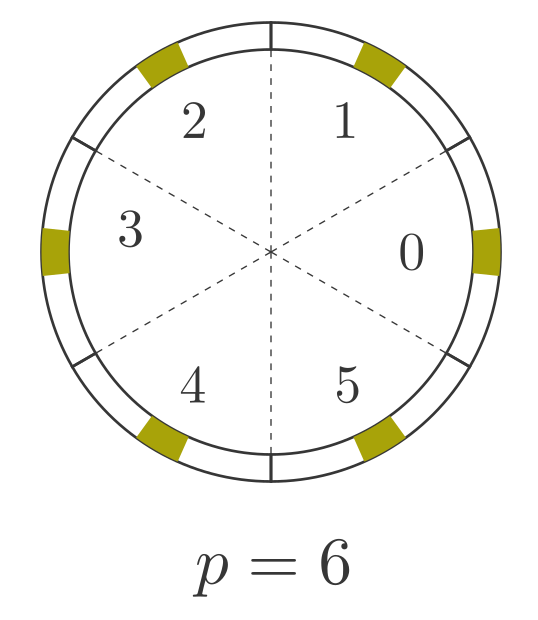
\includegraphics[width=0.8\textwidth]{img/to_harmonize/busy_sectors_2.png}
	\end{minipage}
	\hspace{0.04\textwidth}
	\begin{minipage}{0.47\textwidth}
		\centering
		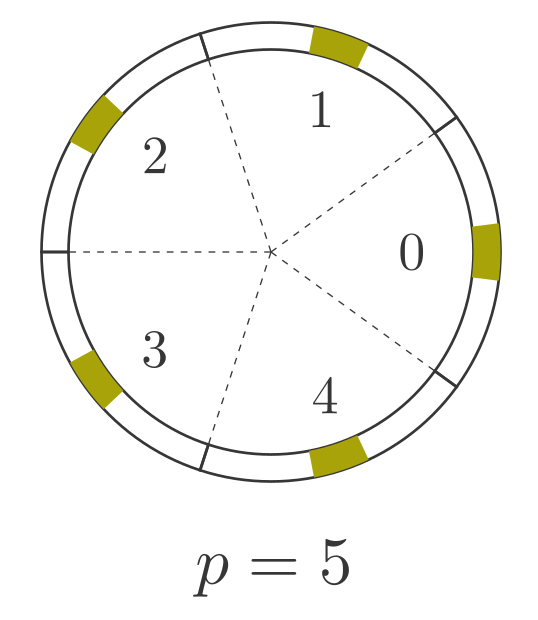
\includegraphics[width=0.8\textwidth]{img/to_harmonize/busy_sectors.png}
	\end{minipage}
	\caption{Distribution of the values of $\mu$ across $\mathbb{Z}_q$ for $p = 6$ and $p = 5$: the colored parts show the dense spots where the value has a high probability to lie in. The width of these sectors depends on $\sigma$ (the standard deviation of the error distribution $\chi$ of TFHE). Note that this repartition looks similar for $\Tilde{\mu}$ in $\mathbb{Z}_{2N}$.}
	\label{fig:density_of_phase}
\end{figure}


When we transpose these dense spots into $\Z_{2N}$, they become the sectors close to $\left \{ \rounding{\frac{k \cdot 2N}{p}} \mid k \in \Z_p \right \}$. 

Let $k \in \Z_p$, the multiplication $X^{- \frac{k \cdot 2N}{p}} \cdot v(X)$ in the ring $\glweRing$ yields the same degree-zero coefficient as the multiplication  $X^{\modulo{- \frac{k \cdot 2N}{p} + N}{2N}} \cdot v(X)$, up to the minus sign. To make the rest of this section clearer, we change a bit the writing of the exponent as such: 
\[\modulo{
	\frac{
		-k \cdot 2N
	}
	{
		p
	}
	+ N
}{2N} = 
\modulo{
	\frac{
		(-k + \frac p 2 ) \cdot 2N
	}
	{p}
}
{2N}\]


This is where the parity of $p$ plays a part: if $p$ is even, then $\modulo{
	\frac{
		(-k + \frac p 2 ) \cdot 2N
	}
	{p}
}
{2N}$ is a dense spot as well. So collisions happens with high probability.  On the other hand, let us consider an odd value for $p$. Then, $\modulo{
	\frac{
		(-k + \frac p 2 ) \cdot 2N
	}
	{p}
}{2N}$ is no longer a dense spot, as it lies exactly halfway between the two dense spots $\modulo{
	\frac{
		(-k + \frac {p-1} {2} ) \cdot 2N
	}
	{p}
}{2N}$ and $\modulo{
	\frac{
		(-k + \frac {p+1} {2} ) \cdot 2N
	}
	{p}
}{2N}$. As a consequence, collision never occurs. Figure \ref{fig:torus_p_even_vs_odd} illustrates this phenomenon.


\begin{figure}
	\begin{subfigure}{0.49\linewidth}
		    \centering
		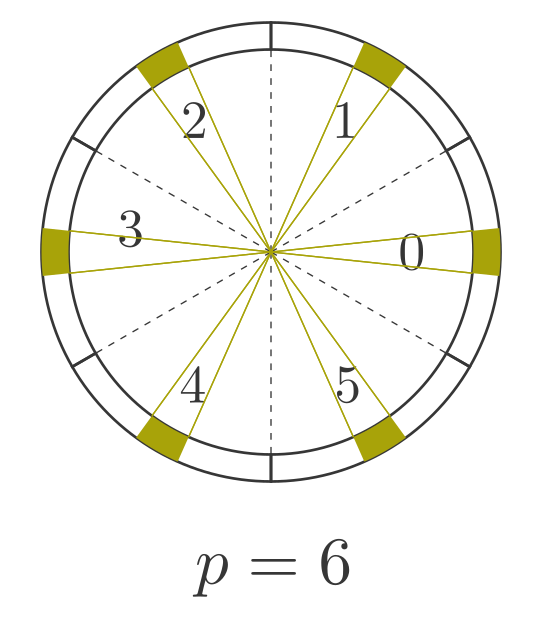
\includegraphics[width=0.5\linewidth]{img/to_harmonize/torus_p_even.png}
		\caption{With $p$ even, the dense spots of each half of the torus are aligned.}
		\label{fig:torus_p_even}
	\end{subfigure}\hspace{1em}% Adjust the margin width as needed
	\begin{subfigure}{0.49\linewidth}
		\centering
		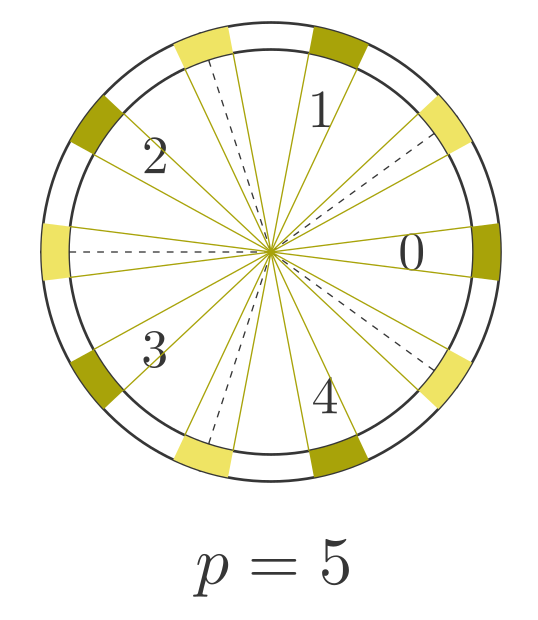
\includegraphics[width=0.5\linewidth]{img/to_harmonize/torus_p_odd.png}
		\caption{With $p$ odd, the dense spots face empty spots, close to the bounds of the $p$-sectors.}
	\end{subfigure}
	\caption{}
	\label{fig:torus_p_even_vs_odd}
\end{figure}



So, by selecting odd values for the plaintext modulus, the negacyclicity problem is naturally neutralized.


We present in Definition \ref{def:odd_accumulator} the formula for the accumulator in this case. Note that because $N$ is a power of two and $p$ an odd value, some rounding is required in the quotient $\frac N p$, but we omit it to keep notations lighter, (or )equivalently, the division operator is assumed to include rounding).

\begin{definition}(Odd-case Accumulator)
	\label{def:odd_accumulator}
	Let $p$ and $p'$ be two integers, with $p$ \textbf{odd}. Let $f: \Z_p \mapsto \Z_{p'}$ a function, and $N$ a power of two. Then, the accumulator $\acc \in \glweRing$ has the form:
	\[
		\acc^{\textsf{odd-modulus}} = X^{- \frac {N} {2p}} \cdot \sum_{j=0}^{N/p - 1} X^j  \cdot \left ( \sum_{i=0}^{\frac{p-1}{2}} f(i) X^{i \frac{2N}{p}} + \sum_{i=0}^{\frac{p-1}{2} - 1} -f \left (i + \frac{p+1}{2} \right ) X^{i \frac{2N}{p} + \frac N p} \right )
	\]
	
	\paragraph{Remark on the encoding:}
	With this construction, we do not need a bit of padding anymore. So, the values $f(i)$ are encoded using the simple encoding of Section \ref{sec:encryption}, that is to say $\rounding{\frac{f(i) \cdot q}{p}}$.
\end{definition}



Let us explain the structure of this accumulator. The polynomial has degree $N$ and is made of $p$ distinct windows of width $\frac{N}{p}$. Each of these windows has constant coefficient value $f(k)$, for $k \in \{0, \dots, p-1\}$.
For $0 \le \alpha \le \frac{p-1}{2}$, the range of degrees whose coefficients are $f(\alpha)$ is $\left [ \alpha \frac{2N}{p} - \frac{N}{2p}~;~ \alpha \frac{2N}{p} + \frac{N}{2p} \right ]$. Now, for $\frac{p+1}{2} \le \beta \le p-1$, we can write $\beta = \alpha + \frac{p+1}{2}$, with $0 \le \alpha < \frac{p-1}{2}$. This time, the range of spanned degrees is $\left [ \alpha \frac{2N}{p} + \frac{N}{2p} ~;~ (\alpha + 1) \frac{2N}{p} - \frac{N}{2p} \right ]$. Thus, the values $k \in \{0, \dots, p-1\}$ spans the entire space $[0; N)$ without overlap. The values over $\frac{p+1}{2}$ gets negated by the negacyclicity, so the underlying coefficient is also negated to compensate this effect. We illustrate this construction on Figure \ref{fig:accumulator_odd}.




\begin{figure}[H]
	\centering
	
\begin{tikzpicture}
		\drawSingleRing{5}{5}{small}{true}{true}{true}
		\drawRingOddEncoding{64}{5}{big}{true}{false}
		\draw[red, loosely dashed, line width=1mm] (-6,0) -- (6,0);
	\end{tikzpicture}
	
	\vspace{1.5em}
%	
	\textbf{Odd-Modulus Accumulator:}\\[0.5em]
	\oddAccumulator{5}{32}
%	
%	\vspace{1.5em}
%	\textbf{Rotated by $N$:}\\
%	\oddAccumulatorInverted{5}{32}
	\caption{Illustration of the construction of the Odd-Modulus accumulator. On top is the ring $\Z_{2N}$ splitted in windows. Below is a representation of the polynomial $v$, with its version once rotated by a multiplication by $X^N$. On the figure, $p = 5$ and $N = 32$. Hatching shows the parts which have an additional minus signs}
	\label{fig:accumulator_odd}
\end{figure}


If we compare this approach to the bit-of-padding one, the windows have half the size. So we may think that the bound on the maximal noise to ensure correctness must be twice tighter. However, because the bit-of-padding accumulator makes use of only one half of the torus, the windows actually have the same width if we consider the same size of plaintext space. In Section \ref{sec:parametrization}, we elaborate further on how the parametrization of the scheme is handled in this case.


With this technique, no bit of padding is required. Consequently, it allows to use the linear homomorphisms without worrying about carry propagation. This is a key improvement that is at the root of the works presented in the rest of this thesis.




\section{Other countermeasures avoiding the bit of padding}
\label{sec:soa_padding_bit}

Because the classical bit-of-padding solution brings too many constraints on the evaluation of computational circuits, several alternative constructions have been proposed to homomorphiclaly evaluate LUT. To do so, many of these constructions adopt a similar strategy: they decompose the target function into a sequence of several PBS steps. 

A notable line of work, including \cite{EPRINT:YXSCZ21}, \cite{AC:LiuMicPol22}, and \cite{TCHES:KluSch23}, employs a two-step PBS strategy. In these approaches, the first PBS evaluates a quantity  encrypting the bit indicating whether the message lies in the positive or negative half of the torus. This effectively extracts the ``sign'' of the message. The second PBS then evaluates the actual function of interest regardless of the effects of negacyclicity, producing a result that may be flipped in sign. The ambiguity introduced by this flip is corrected using the result of the first PBS. While the specific techniques used to perform this correction vary across works, the overall architecture remains the same: use the first PBS to identify the torus half, and use this information to rectify the sign of the second PBS output.

Another interesting approach is presented in \cite{AFRICACRYPT:CBSZ23}, where the target function is expressed as a sum of functions sharing a particular structure: so-called \textit{pseudo-odd} and a \textit{pseudo-even} function. These two properties are special cases of negacyclic functions, so they allow an evaluation with a PBS without suffering from the negacyclicity issue. Although this decomposition may require more than two PBS calls, an important advantage of the method is that the evaluations can be carried out in parallel. This contrasts with the previously mentioned approaches, which are intrinsically sequential due to the dependency between the two PBS stages.

A completely different line of work is explored in \cite{AC:CLOT21}, which introduces the “Without-Padding PBS” (WoP-PBS) construction. A more refined version of this technique is presented in \cite{JC:BBBCLO23}, and we describe it here. The method begins by evaluating a scaled sign function (that is inherently negacyclic) using a standard PBS. Following this, the individual bits of the message are extracted and converted into $\GGSW$ ciphertexts (see Definitions \ref{def:ggsw} and \ref{def:ggsw2}) using a procedure known as \textit{circuit bootstrapping}. These ciphertexts are then used as selectors in a graph of $\CMUX$ operations (Definition \ref{def:cmux}) to select an appropriate accumulator based on the high-order bits of the message. Finally, a traditional PBS is used to rotate the selected accumulator according to the remaining lower-order bits.

Although this technique is slower for small plaintext sizes, it scales particularly well with increasing input sizes. Notably, it enables the homomorphic evaluation of LUTs with larger plaintext sizes beyond what is feasible with classical PBS techniques, up to approximately 20 input bits.


Our idea of employing odd plaintext moduli that we developed in Section \ref{sec:odd_modulus} do not have any computational overhead with respect to the classical bit-of-padding (contrary to the other approaches we presented in this section), while removing all the constraints the latter put on the homomorphic compilation. However, working with an odd modulus may seem unhandy: data types in programming are usually defined on a power-of-two modulus for example.

Chapter \ref{chap:p_encodings}, \ref{chap:hyppogriph}, \ref{chap:transistor} and \ref{chap:larger_lut} are examples of applications enabled by this feature of odd plaintext modulus.

